\documentclass[11pt,a4paper]{article}

\usepackage{graphicx}
\usepackage{caption}
\usepackage{fullpage}

\begin{document}
\title{%
  \large Paper Reading:\\
  \Large \textbf{Audio-Video Sensor Fusion with Probabilistic Graphical Models}\\
  \large by Matthew J. Beal, Hagai Attias, and Nebojsa Jojic\\
  \large in \textit{ECCV 2002}
}
\author{Weipeng He}
\date{\today}
\maketitle

\section{Introduction}

This paper addresses a probabilistic graphical model approach for audio-visual object tracking. More precisely, the approach is applied for tracking person talking and moving. Sensor data are collected by a camera and two microphones.

They claim that most previous systems treat audio and video data separately and then combine them at higher level. These previous systems are subject to scenario dependency and requires complicated calibration procedure. To tackle these issues, they propose a graphical-model-based system that exploits the correlations among audio-visual signals by directly describing the joint distribution of the two modalities.

\section{Approach}

Their proposed approach can be described using the graphical model in Fig.~\ref{fig:model}. 

\begin{figure}
  \centering
  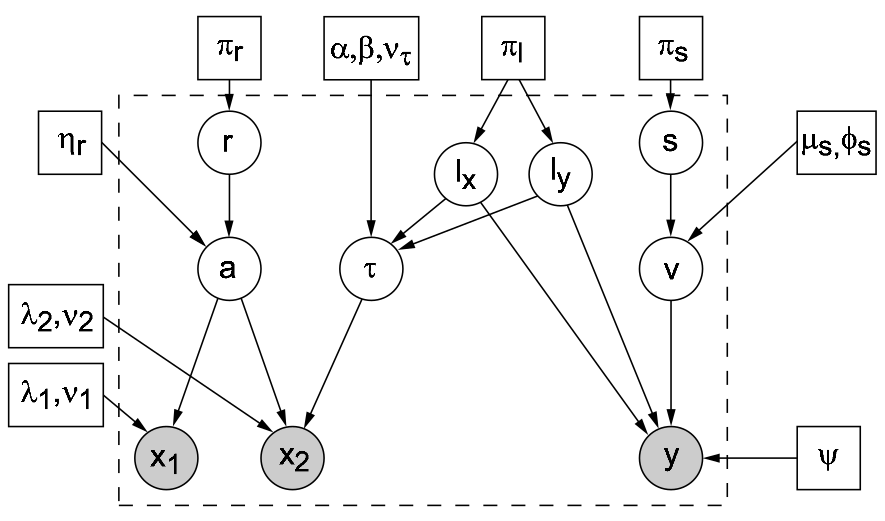
\includegraphics[width=0.6\textwidth]{model}
  \caption{The proposed graphical model.}
  \label{fig:model}
\end{figure}

In the graph, $x_1, x_2$ are the audio observations (2 channel time-domain signal) and $y$ is the visual observation (gray scale image).
The audio observation is Gaussian around $a$ (source audio signal) with attenuation and delay $\tau$ (for $x_2$). $a$ is a Gaussian Mixture. The visual observation is Gaussian around $v$ (visual template) shifted by the object position $l$.

The audio and visual information is fused via the linear correlation between $\tau$ and $l$. And the correlation parameters are part of the model parameters, therefore the calibration is automatically done by learning.

They use the expectation-maximization algorithm to estimate the model parameters and the object position (which is a hidden variable) is estimated by maximizing its posterior probability.

\section{Experiment}

The proposed approach is tested on two video recordings with substantial audio and visual noise and compared to unimodal methods. The result shows that the audio-visual fusion method achieves good tracking performance and significantly outperforms unimodal methods. The result is shown in Fig.~\ref{fig:result}.

\begin{figure}
  \centering
  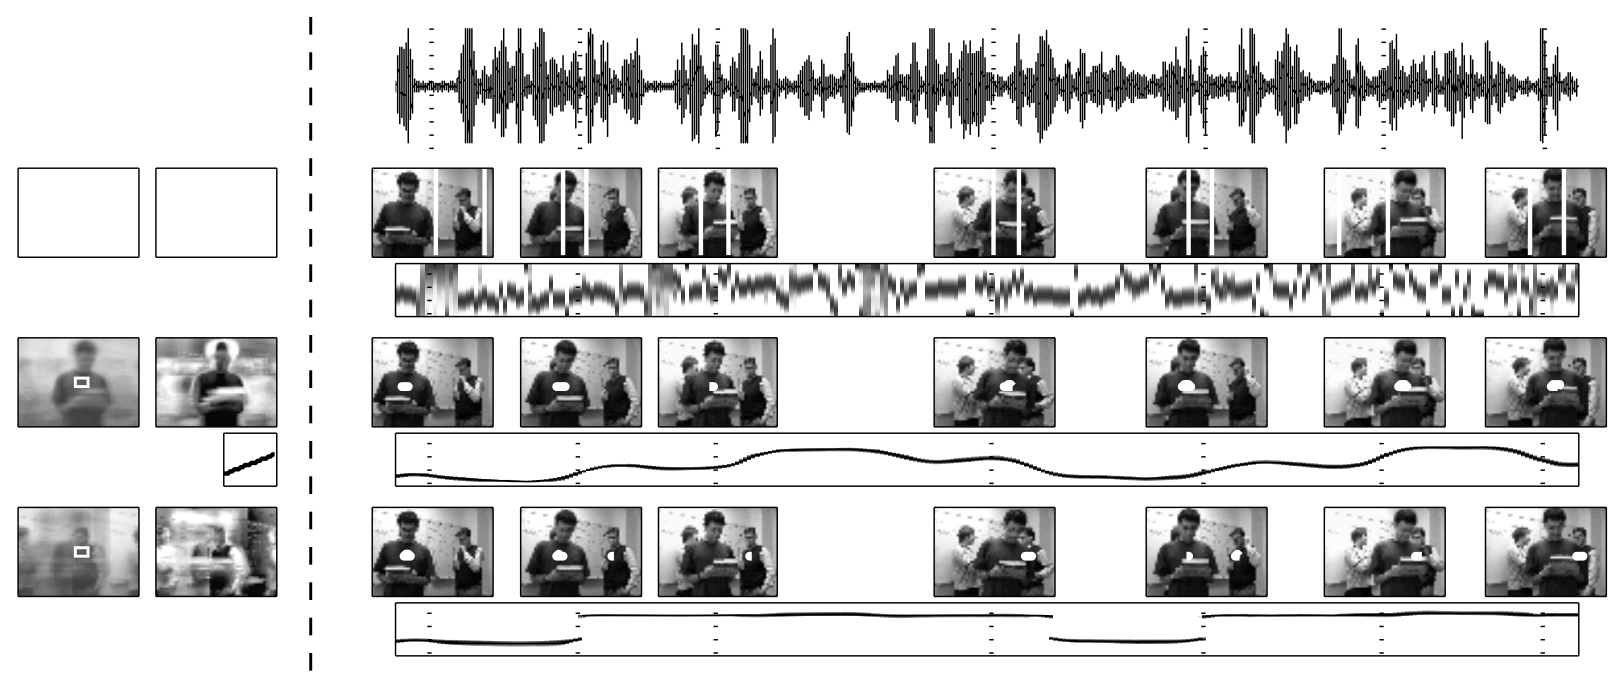
\includegraphics[width=.8\textwidth]{result}
  \caption{Experiment result.}
  \label{fig:result}
\end{figure}

\section{Conclusion}

The conclusions in the paper can be summarized as:

\begin{itemize}
  \item The system does not require special calibration procedure.
  \item No temporal filtering is needed and therefore the system is robust to sudden movements.
  \item Using generative model, it is able to explain noises and making the trajectory smooth.
\end{itemize}

\section{Discussion}

Overall, this paper shows a novel approach and its performance is justified by the experiments. However, some of the conclusion is trivial or not convincing. For instance, the system is actually doing detection rather than tracking, so it is obvious that the system will be robust to sudden movements. Additionally, I do not agree with that the system's ability to tackle noise is because the generative model. By using discriminative methods it is also possible to handle noise. Furthermore, the visual observation model is not invariant to scaling, which is actually quite important in practical systems.

What I found very interesting but not mentioned in the paper is that: they have not used any labeled data. They do the ``tracking'' with completely unsupervised learning. Even the visual template is learned, by the heuristic of audio-visual correlation. This is a good example of multi-modality fusion that helps each other.

\end{document}

